%%%%%%%%%%%%%%%%%%%%%%%%%%%%%%%%%%%%%%%%%%%%%%%%%%%%%%%%%%%%%%%%%%%%%%%%%
%
% This file defines the style for your homebook
% You don't need to edit it any more, if not to 
% change the authors name:
%
% Search below for the keyword:   GROUP
% insert your group number
%
% Search below for the keyword:   AUTHORS
% insert the name of the authors
%
%%%%%%
% Now to update the dexcription  of your work you will 
% use the file ``master.tex'' in the current directory
% following the instructions in it 
%
%%%%%% 
%%%%%%  
%%%%%%
% If you want to compile your document you have TWO ways
% depending on the fact that 
% 	1) you have inserted only postcript images in your tex file 
%		---> then go to MODE 1
%	2) you have inserted other kind of images (jpg..) in your tec file
%		---> then go to MODE 2
%
% MODE 1 
%simple type:
% 	latex homebook.tex
%
% If the compilation runs succesfully and you want to see the results type:
% 	xdvi homebook.dvi &
% and use the menus to go through the document
%
% If you want to create a pdf type:
% 	dvipdfm homebook.dvi
%
% a homebook.pdf file is created
% you can see it using the command:
% 	acroread homebook.pdf &
%
%
% MODE 2
% simple type:
%	pdflatex homebook.tex
%
% If the compilation runs succesfully you directly have the pdf file
% and you can see it using the command:
%       acroread homebook.pdf &
%
% 
%%%%%%%%%%%%%%%%%%%%%%%%%%%%%%%%%%%%%%%%%%%%%%%%%%%%%%%%%%%%%%%%%%%%%%%%%%
\documentclass[10pt,  english, makeidx, a4paper, titlepage, oneside]{book}
\usepackage{babel}
\usepackage{fancyhdr}
\usepackage{makeidx}
\usepackage{titlesec}
\usepackage{listings} 


\newenvironment{listato}{\footnotesize}
                        {\normalsize }


%\pagestyle{empty}

\textwidth 15.5cm
\textheight 23cm
\topmargin -1cm
\oddsidemargin -0.5cm
\linespread{1.1}

\pagestyle{fancy}
\lhead{}
\chead{Integrated Systems Architecture}
\lfoot{}
\cfoot{}
\rfoot{}
\rhead{\thepage}

\usepackage{graphicx}
\usepackage{amsmath}
\usepackage{amsfonts}
\usepackage{amsthm}
\usepackage{amssymb}
%\oddsidemargin -1.1cm

\titleformat{\chapter}[display]
{\normalfont\Large\filcenter\sffamily}
{\titlerule[0.5pt]%
\vspace{1pt}
\titlerule
\vspace{1pc}
\LARGE\MakeUppercase{\chaptertitlename} \thechapter
}
{1pc}
{\titlerule
\vspace{1pc}
\Huge}

\newcommand{\SubSubSection}[1]{\subsubsection{\bf Exercise   ~#1}}

\newcommand{\homework}[1]{\subsubsection{\bf Homework   ~#1}}

\newcommand{\Solution}{\subsubsection{\bf Solution}}




\makeindex
\begin{document}
\frontmatter
\begin{titlepage}
\vspace{2cm}
\centerline{

\includegraphics[width=2cm]{./logopoli}}  
\centerline{\LARGE Politecnico di Torino}
\bigskip
\centerline{\Large III Facolt\`a di Ingegneria}
\vspace{4cm}
\centerline{\Huge\sf Exercises and Homeworks for the course}
\bigskip
\centerline{\Huge\bfseries\sf Integrated Systems Architecture}
\vspace{2cm}
\centerline{\LARGE Master degree in Electrical Engineering}
\vspace{4.4cm}
%%%%%%%%%%%%%%%%%%%%%%%%%%%%%%%%%%%%%%%%%%%%%%%%%%%%%%%
% GROUP
% Change the name of your group below
%
\centerline{\Large Authors: e02GQCxx}
\vspace{2cm}
%
%%%%%%%%%%%%%%%%%%%%%%%%%%%%%%%%%%%%%%%%%%%%%%%%%%%%%%%
% AUTHORS
% Change the name of the Group participants here
%
\centerline{Paperoga, Gilberto de Pippis, Brigitta, Filo Sganga}
%
%%%%%%%%%%%%%%%%%%%%%%%%%%%%%%%%%%%%%%%%%%%%%%%%%%%%%%
\vspace{2cm}
\centerline{\today}
\vspace{1cm}
{\scriptsize Many thanks to Prof. Mariagrazia Graziano for providing us with this template.}
\end{titlepage}

\tableofcontents

%%%%%%%%%%%%%%%%%%%%%%%%%%%
% 
\mainmatter
\lstset{language=VHDL}

%%%%%%%%%%%%%%%%%%%%%%%%%%%%%%%%%%%%%
%%%%%%%%%%%%%%%%%%%%%%%%%%%%%%%%%%%%%
%%    
%% HERE IS THE MAIN INCLUSION
%%
\chapter{Datapath}
We have implemented the VHDL architecture of the processor(Figure \ref{fig1}), splitted in 5 pipeline stages: \\
Fetch, Decode, Execute, Mem, WriteBack. \\
Instructions and datas of the entire procssor are represented on 32 bits. 
\begin{figure}[h!]
	\centering
	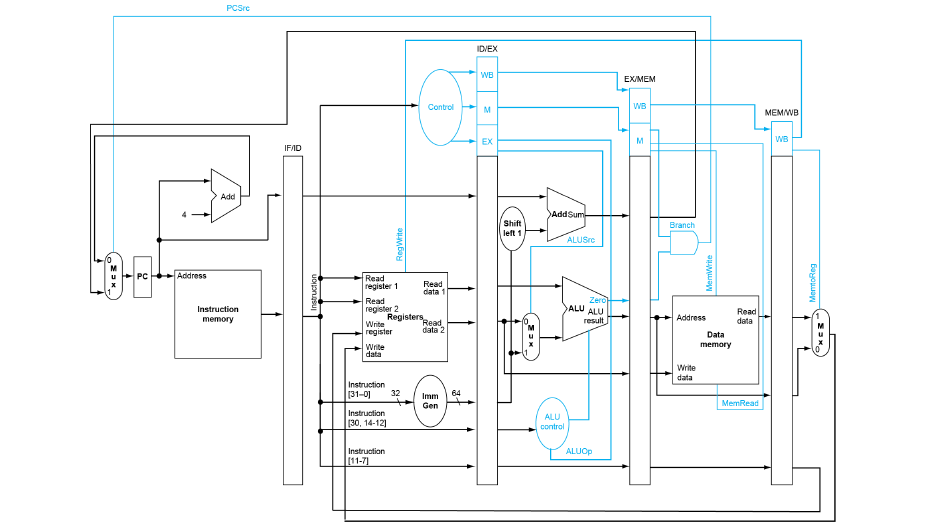
\includegraphics[width=18cm]{./images/structure}
	\caption{General structure}
	\label{fig1}
\end{figure}
As specification says, Instruction and Data memory was not included. We have implemented it in the testbench.\\
Here we have tried to impement most of the single blocks in a Structural way. \\
Only Register file, alu and all filpflops are implemented as Behavioral.\\
\\
On Figure \ref{fig2} it is showed how we have organized the VHDL files.
\begin{figure}[h!]
	\centering
	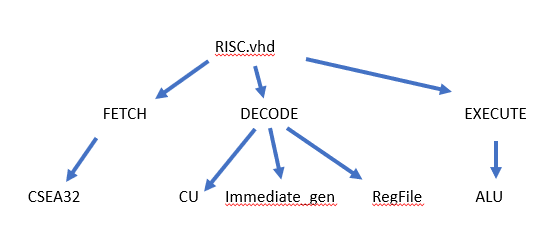
\includegraphics[width=15cm]{./images/VHDL_structure}
	\caption{General VHDL structure}
	\label{fig2}
\end{figure}
Now more details on singolar block implementation.
\section{Fetch}
\begin{figure}[h!]
	\centering
	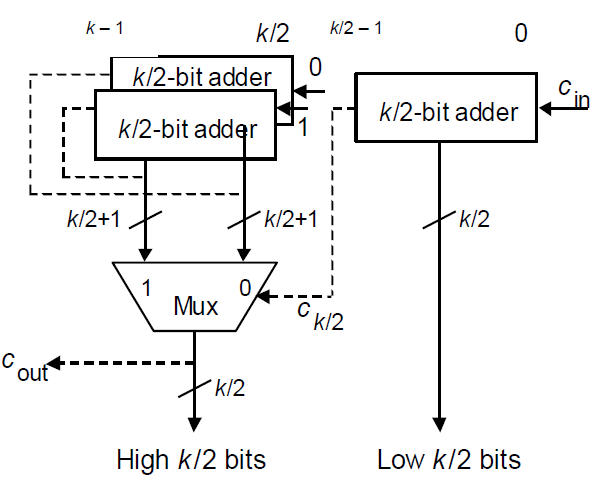
\includegraphics[width=10cm]{./images/CSEA}
	\caption{CSEA structure}
	\label{fig3}
\end{figure}
To update the PC we have implemented a Carry Select Adder. \\
Each singolar blocks are compose of a 8 bit Ripple carry adder. In this way we have reduced the delay.
\section{Decode}
The register file is behavioral. It's composed of 32 registers on 32 bits. \\
At each rising edge of the clock, read two value given the addresses Register\_read1 and 2.\\
If the write enable is 1, we write in the register location.
It have this port:
\begin{itemize}
	\item Write enable port;
	\item Register read1;
	\item Register read2;
	\item Write register;
	\item Write data;
	\item Read Data1;
	\item Read Data1;
	\item Clock;
	\item Reset;		
\end{itemize}

The Immediate\_generate block read the instruction and generate the Immediate value.
\begin{figure}[h!]
	\centering
	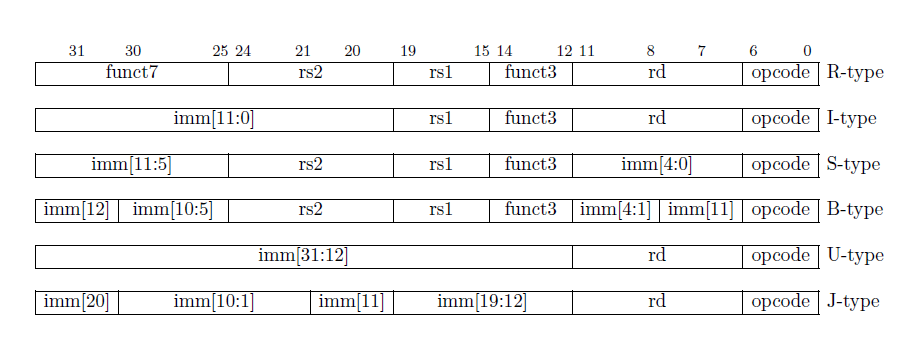
\includegraphics[width=10cm]{./images/immediate_gen}
	\caption{Instruction organization}
	\label{fig4}
\end{figure} 
So based on which instruction we are decoding, organize a 32 bits Immediate value.
\section{Execute}
The adder that create the new program counter is again implemented with a 32 bits CSEA.
Then we have the Alu that receive two inputs value and the Opcode specify which instruction implement.
\section{Memory}
This module is implemented in the RISC top entity. Contain only the AND port that generate the selection signal for the multiplexer on the fetch phase.
\section{Write back}
This module is implemented in the RISC top entity. Contain a multiplexer of 4 inputs and decide between:
\begin{itemize}
	\item Data memory read;
	\item Alu result;
	\item PC + 4 taken from fetch unit;
	\item PC where we need to jump;
\end{itemize}
The last two inputs are considered for the instruction auipc and jal.
For the JAL stores the address of the instruction following the jump (pc+4) into register rd.\\
So we take the updated PC in the fetch phase and we bring it in the Write Back phase.\\
AUIPC forms a 32-bit offset from the 20-bit U-immediate, adds this offset to the address of the AUIPC instruction.\\
Then places the result in register rd. 
We take the result in the Execute phase, where with the CSEA we create the branch PC.
%%
%% NOW READ THE FILE master.tex  
\end{document}

